\chapter{Preliminary}
\label{chap:02-preliminary}

This chapter presents the preliminary knowledge needed to understand the research detailed in the remainder of this thesis. More precisely, it covers what anomalies are in time-series, a taxonomy of existing anomaly detection methods for time-series, and a theoretical breakdown of how Generative Adversarial Networks work.

% ----------------------------------------------
\section{Anomaly Detection for Time-Series}
\label{sec:ad-for-ts}
% ----------------------------------------------
Before digging into the how, we should be able to answer the what, and more precisely, what is an anomaly? There is no precise definition for an anomaly, but it is well accepted as an observation that differs significantly from the rest of the distribution, suggesting that a different mechanism might have generated it than the rest of the data \cite{hawkins1980iden_outliers}. It is an ill-posed problem because the solution depends heavily on the definition of an anomaly in the specific domain being analyzed, and the result may not be unique. For instance, in the context of stock data, a sudden change in the mean of the data indicates an external political, social, or economic event that changed it forever, whereas in healthcare monitoring, it might suggest an emergency that calls for action. 

Another problem that might arise in anomaly detection is confusing measurement noise with outliers. Among the areas where this confusion can appear are sensor settings, network telemetry, and industrial monitoring, where an expert should sanitize the data before running any learning procedure. With an in-depth understanding of the system's normal behavior, the expert can fit the data into a probability distribution and then identify anomalies by measuring how much they deviate from the mean of that distribution. Moreover, if previous anomalies are available, the problem can be solved with a supervised method, where more knowledge can be incorporated. However, in real-world scenarios, the underlying distributions are often difficult to identify due to the complexity of the data, which creates the need for unsupervised learning methods. All learning paradigms can be meaningful in anomaly detection, but unsupervised methods are especially useful because they make use of the large amount of unlabeled datasets.  

In time-series, an anomaly can be broadly separated into two categories: point anomaly and collective (sequence) anomaly \cite{boniol2024ts-ad-review}. A point anomaly can be either global, when a value falls outside the normal range of values of the entire time-series, or contextual, when it is unusual only within the local neighborhood values around that point. More complex, a collective anomaly is a collection of consecutive data points that do not resemble normal behavior. An example of where collective anomalies appear is in the domain of fraud detection, in which a set of successive actions defines the fraud itself, such as logging in at an unusual time, sending money to an account without previous interaction, and deleting the trace. An illustration of these categories can be seen in the Figure \ref{fig:ts-anomaly-types}, where all types of anomalies are showcased: a global point anomaly (a) where the value is outside the expected global range of values, a contextual point anomaly (b) where the value is outside the expected local range of values, and a sequence anomaly (c) where the variance of the sequence is abnormal, but its values are inside the normal range \cite{boniol2024ts-ad-review}.

\begin{figure}[H]
    \centering
    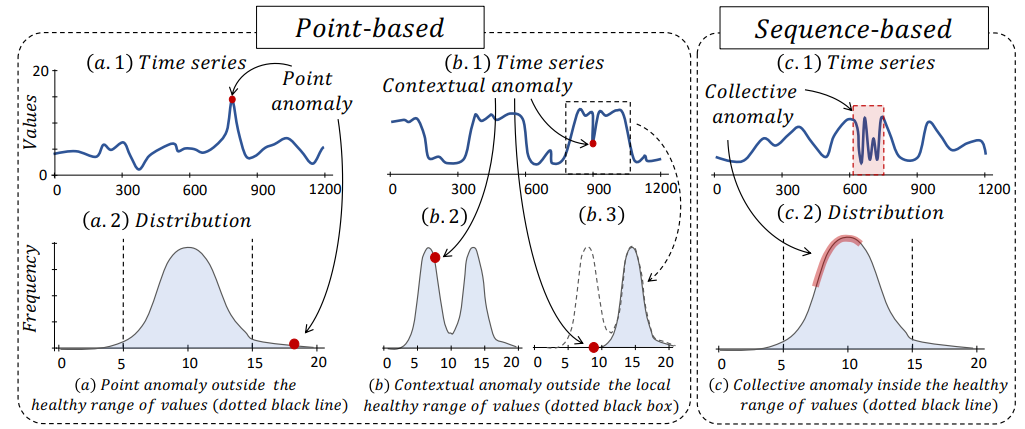
\includegraphics[width=0.75\linewidth]{images/02_ts_anomalies.png}
    \caption{Point-Based and Sequence-Based Anomalies. Source \cite{boniol2024ts-ad-review}.}
    \label{fig:ts-anomaly-types}
\end{figure}

In \cite{boniol2024ts-ad-review}, a taxonomy for time-series anomaly detection methods was presented, which divided the methods into three categories: distance-based, density-based, and prediction-based. Given that most of the methods are unsupervised, this provides a clearer taxonomy for comparing anomaly detection algorithms than separating them into supervised, semi-supervised, and unsupervised categories. Thus, in the following subsections, the taxonomy defined in \cite{boniol2024ts-ad-review} will be discussed in detail, with the focus of presenting the base methods from which the state-of-the-art was built upon for each category.

\subsection{Notations and Terminology}
\label{subsec:2.1.1-notations-and-terminology}

There are many different notation styles for time-series data, especially when describing reconstruction-based or forecasting-based methods. Thus, in this subsection, we define the notations and terminology used throughout this thesis.

A multivariate time-series is denoted by $X = \{x_1, x_2, \ldots, x_T\} \in \mathbb{R}^{T \times M}$, where each observation $x_i \in \mathbb{R}^{M}$ represents a vector of $M$ features at time step $i$, and $T$ is the total length of the series. 

For methods that operate on local temporal windows, the time-series is transformed into a set of overlapping subsequences using a sliding window of size $s_w$ and a step size $s_s$. The new set of subsequences is denoted by $\textbf{X} = \{\textbf{x}_1, \textbf{x}_2, \ldots, \textbf{x}_N\}$, with $\textbf{x}_i \in \mathbb{R}^{s_w \times M}$ and $N = \lfloor \frac{T - s_w}{s_s} \rfloor  + 1$. For methods using a latent space, the latent space is denoted by $Z$ and its dimension by $z_w$.

A time-series that was built by aggregating forecasts or reconstructions is denoted by $ \tilde{X} = \{\tilde{x_1}, \tilde{x_2}, \dots, \tilde{x_T}\} \in \mathbb{R}^{T \times M}$, where $\tilde{x} \in \mathbb{R}^{M}$, with the same size as $X$.

\subsection{Distance-based}
The distance-based methods directly use the values of a time-series as they are, without accounting for the trend and seasonality of the data. These methods detect anomalies solely using distance measurements. Given two time-series $A, B \in \mathbb{R}^{T \times M}$, where $T$ denotes the number of time steps and $M$ the number of features, the distance between them is denoted as $d(A, B)$ and the most common distances used are the Euclidean or Manhattan distance, or more generally, any Minkowski distance.

We mention that among the earliest methods used to detect anomalies in time-series is k-th Nearest Neighbours (KNN) \cite{angiulli2002knn-ad}. Using the distance metric $d(\cdot)$, KNN looks at the closest $k$ neighbours of an object, and depending on the task, it uses those distances for classification, regression, or anomaly detection. For time-series, the algorithm divides the time-series into subsequences, for which it computes the anomaly score by aggregating the distance to its closest k-neighbours in different ways: mean, median, minimum, or maximum. KnorrSeq2 is a variant of KNN introduced in \cite{palshikar2005knorrseq} that looks at the $k$ previous or the $k$ following sub-sequences, and labels a sub-sequence as an anomaly if at least $p\%$ of its neighbours are at a distance larger than a threshold $D$.

Another popular distance-based method is the Local Outlier Factor (LOF) \cite{breunig2000lof}, which poses the following question: how dense is the local neighbourhood of this point compared to the density of its neighbours?. To answer this question, a measurement of the local reachability distance of a point was defined. Let $k\text{-}dist(A)$ be the distance from $A$ to its $k$ nearest neighbour, let $N_k(A)$ be the set of the $k$ nearest neighbours of A, and let $reach\text{-}dist_k(A, B) = max\{k\text{-}dist(B)\text{, } dist(A, B)\}$ be the reachability distance from point B to A, but this distance needs to be at least $k\text{-}dist(B)$. The $reach\text{-}dist_k(A, B)$ distance ensures if the point $A$ is in the $k$ proximity of point $B$, where $B$ is a point in the $k$ proximity of $A$. Finally, the local reachability distance of a point $A$ can be defined as the inverse of the average reachability distance of the point $A$ from its neighbours \cite{breunig2000lof}:
$$ 
lrd_k(A) = \left(\frac{\sum_{B \in N_k(A)} reach\text{-}dist(A, B)}{|N_k(A)|}\right)^{-1} 
$$
Using $lrd_k(\cdot)$, an anomaly score can be computed for a point $A$ by comparing $lrd_k(A)$ with $lrd_k(B), \forall B \in N_k(A)$. If the anomaly score is $\sim 1$, then the local density of $A$ is very close to the local densities of its neighbours, and it is considered a normal point; otherwise, as the score gets bigger, $A$ is much closer to being an anomaly. Intuitively, LOF assigns a high anomaly score to points that lie in regions significantly less dense than their neighbors. In the context of time-series data, the pipeline is identical to the one used for KNN: the time-series is divided into smaller sub-sequences, and we are interested in comparing the local reachability of these sub-sequences.

\subsection{Density-based}
Density-based methods capture complex correlations within the data by modeling the underlying density of subsequences. These approaches can be divided into four categories: graph, encoding, distribution, and tree-based methods \cite{boniol2024ts-ad-review}. We focus our attention on distribution and tree-based approaches.

Distribution-based algorithms build statistical models from subsequences of the time-series, aiming at finding their underlying distribution. Most of the distribution-based methods are based on the Support Vector Machine (SVM) learning algorithm \cite{boniol2024ts-ad-review}, and one such popular method is the One-Class SVM (OC-SVM) \cite{scholkopf1999oc-svm}. OC-SVM separates the data from the origin with maximum margin, effectively capturing the region where normal
OC-SVM searches for a maximum margin hyperplane that separates the data from the origin, learning where normal instances reside in a high-dimensional feature space induced by a kernel function. It is mandatory to train the algorithm with normal time-series that do not contain any anomalies, which makes OC-SVM a semi-supervised approach. The fraction of allowed anomalies during training is controlled by the hyperparameter $\nu$, which makes the method robust to small amounts of contamination in the training data. Thus, given subsequences $\{ \textbf{x}_1, \textbf{x}_2, \dots, \textbf{x}_N \}$, OC-SVM solves:
$$
\min_{w, \rho, \xi} \frac{1}{2} ||w||^2 + \frac{1}{\nu N} \sum_{i=1}^N \xi_i-\rho
$$
$$
\text{subject to } w \cdot \phi(\textbf{x}_i) \geq\rho - \xi_i, \xi_i \geq 0,
$$
where $\phi(\textbf{x}_i)$ is the feature mapping using the kernel function. At test time, samples lying outside the learned boundary are assigned negative scores and considered anomalous.

Tree-based methods work by partitioning the data in a binary tree, aiming to isolate anomalous objects as early as possible. Among them, the most popular method is Isolation Forests (IF), and it is based on the idea that anomalies are "few and different" \cite{liu2008iforest}. The method recursively partitions the data into smaller subsets. Given a dataset $X = \{x_1, x_2, ..., x_N \text{ | } x_i \in \mathbb{R}^M\}$, each split randomly selects a feature $f \in [1,M]$ and a threshold value $v$ sampled from the feature’s observed range: $v \sim \mathcal{U}(f_{min}, f_{max})$ where $f_{min} = \min\limits_{i \in [1,N]} x_i[f]$ and $f_{max} = \max\limits_{i \in [1,N]} x_i[f]$. The data are then split into two subsets, one with $x_i[f] < v$ and the other with $a_i[f] \geq v$, forming a binary tree. Starting from a root node containing all samples, this process continues until a node contains too few samples or the maximum tree depth is reached. Multiple trees are constructed using random subsamples of the dataset, and individual anomaly scores are averaged across the entire forest. Because anomalies require fewer splits to isolate, the final score depends on the average depth of data point $x_i$, normalized by the average path length of an unsuccessful search in a binary search tree \cite{liu2008iforest}. The Extended Isolation Forest (EIF) improves this approach by using random hyperplanes rather than axis-aligned lines to split data points \cite{hariri2019eiforest}. Similarly, the Deep Isolation Forest (DIF) leverages deep learning to introduce non-linearity into the splitting process \cite{xu2023diforest}. Figure \ref{fig:if-eif-dif} compares how IF, EIF, and DIF assign anomaly scores across three distinct dataset shapes, where darker blue regions represent higher anomaly scores.

\begin{figure}[H]
    \centering
    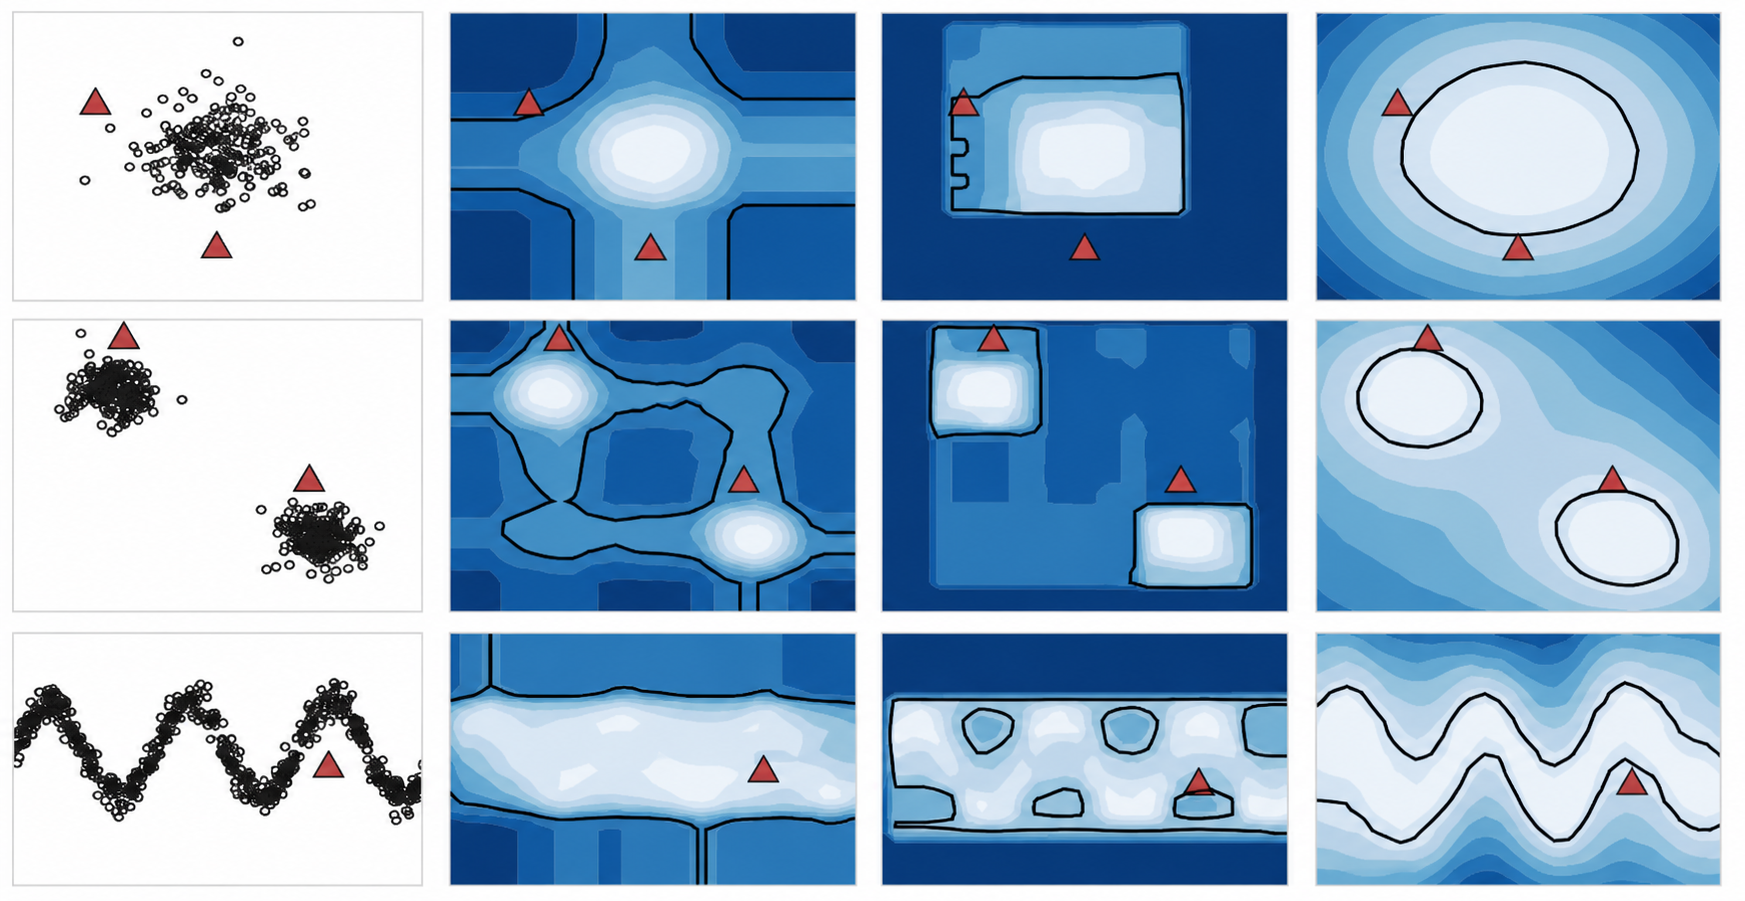
\includegraphics[width=0.75\linewidth]{images/02_if_eif_dif.png}
    \caption{IF vs EIF vs DIF. Source \cite{xu2023diforest}.}
    \label{fig:if-eif-dif}
\end{figure}

\subsection{Prediction-based}
\label{subsec:prediction-based-methods}
Prediction-based methods model normal data behavior under the assumption that anomalies are more difficult to predict. The first category, forecasting-based methods, uses statistical models to predict future time-series values, labeling a point as an anomaly if the difference between the prediction and the true value exceeds a specific threshold. The second category, reconstruction-based methods, compresses data into a lower-dimensional latent space before reconstructing it. Because anomalies lose information during this compression, they are identified by a high reconstruction error.

The Autoregressive Integrated Moving Average, ARIMA\((p,d,q)\), \cite{box2015arima} is a commonly used statistical model for time-series forecasting. The autoregressive part uses the last $p$ values of the series, the moving-average part uses the previous $q$ error terms, and the integrated part refers to differencing the series \(d\) times to make it stationary. It is designed to work for univariate time-series. Thus, setting $M = 1$, we define:
$$
\text{ARIMA}(p,d,q): X_T - \alpha_1 X_{T-1} - \cdots - \alpha_p X_{T-p}
= \varepsilon_T + \theta_1 \varepsilon_{T-1} + \cdots + \theta_q \varepsilon_{T-q},
$$
where $\alpha_i$ denote the autoregressive coefficients, $\theta_i$ the moving-average coefficients and $\varepsilon_i$ the error terms. An anomaly score can be computed from the difference between the ARIMA prediction and the true data. ARIMA is often used as a strong baseline because it assumes a linear relationship in the time-series, while more flexible deep learning methods go beyond this assumption.

Long Short-Term Memory (LSTM) \cite{hochreiter1997lstm} is a recurrent neural network that learns dependencies in sequence data by using gates to decide what to remember, forget, and output at each step. In the context of time-series, it is a forecast-based method that is well-suited for modeling both short and long-term correlations. In \cite{malhotra2015lstm-ad}, a network with two stacked LSTM layers is used to predict $l$ future steps for a subset of $d$ features ($d \le M$) from an $M$-dimensional data point $x_t$, utilizing all $M$ features as context. The model outputs a vector of size $d \times l$, which contains the predictions of $l$ future time steps for each of the $d$ selected features. Based on these predictions, an error vector is computed as $e_t = [e_{11}, e_{12}, \ldots, e_{1l}, \ldots, e_{d1}, e_{d2}, \ldots, e_{dl}]$ and used to fit a multivariate Gaussian distribution $\mathcal{N}(\mu, \Sigma)$. Lastly, a data point is labeled as an anomaly if the likelihood $p_t$ of observing its corresponding error vector $e_t$ under the fitted distribution is below a certain threshold. Although this method assumes that anomalies produce sufficiently large prediction errors, which may not always be true for contextual anomalies, it remains a pivotal work for using LSTM for forecasting and anomaly detection in time-series.

Autoencoders (AEs) are a class of neural networks designed to reconstruct the input data from a lower-dimensional latent space. In this sense, they can be viewed as a nonlinear extension of Principal Component Analysis (PCA). For anomaly detection, the assumption is that an unseen, anomalous subsequence from a time-series will lose information when it is encoded, thus the reconstruction error will be larger. An Autoencoder consists of the encoder $E: \mathbb{R}^{s_w \times M} \to \mathbb{R}^{s_w \times z_w}$ and the decoder $D: \mathbb{R}^{s_w \times z_w} \to \mathbb{R}^{s_w \times M}$, with $z_w << M$ and the reconstruction error will be the point-wise difference $\|\textbf{X} - D(E(\textbf{X}))\|$. EncDec-AD \cite{malhotra2016lstm-enc-dec-ad} utilizes an LSTM network for both its encoder and decoder, aiming to fit a multivariate Gaussian distribution for normal data, thereby extending the previously described method from \cite{malhotra2015lstm-ad}. Other methods \cite{solch2016storn} \cite{park2018lstm-vae-ad} are even using Variational Autoencoders (VAE) for anomaly detection, which, instead of mapping the original data to a latent space, encode inputs as probability distributions.

Finally, the last prediction-based method discussed is Generative Adversarial Networks (GAN), which has two neural networks: the generator and the discriminator. The generator tries to produce realistic samples, while the discriminator learns to distinguish them from real ones. In addition to AEs, GANs have a discriminator that can learn the normality of data from a different perspective, directly posing the question of whether the given input is real or not. To detect anomalies, the reconstruction error is combined with the discriminator score. Subsection \ref{sec:gan} breaks down the theoretical mechanics of the generator and discriminator, while Chapter \ref{chap:03-related-work} shifts the focus to their practical application in time-series anomaly detection.
% ----------------------------------------------


% ----------------------------------------------
\section{Generative Adversarial Networks}
\label{sec:gan}
% ----------------------------------------------

With the growing popularity of deep neural networks in computer vision, which have become state-of-the-art in classification tasks \cite{krizhevsky2012imagenet}, scientists have been enthusiastic about further exploiting the capacities of deep models in other artificial intelligence applications, including object detection, semantic segmentation, and generative models \cite{goodfellow2014gan}.

For the latter, the generative model was trained in an adversarial setting, containing two networks. Given a sample distribution, the task of the generative network was to build new samples that resemble the original distribution, starting from random noise. On the other hand, the adversary network, or commonly named the discriminator, was responsible for detecting if a given object was sampled from the real distribution or if it was counterfeit by the generator.

In this manner, both networks improve their performance: the generator by creating indistinguishable samples from the genuine data, the discriminator by discerning between fake and real data. This unsupervised, adversarial style training, called Generative Adversarial Networks (GAN), is pioneering work for more advanced applications such as image and video synthesis \cite{karras2019style-gan}, image-to-image translation \cite{zhu2017cyclegan}, or medical image augmentation \cite{skandarani2023gan_medical_img}. 

\subsection{Standard GAN}
\label{subsec:standard-gan}

Given a real data distribution $p_X$, the role of the generator is to learn to map the latent space $p_Z$ to the model distribution $p_G$, and to ensure that $p_G$ is aligned with the real distribution $p_X$. The generator is denoted as $G(z;\theta_g)$, where $z$ is the associated latent variable, and $\theta_g$ are the learnable parameters of the generator's deep neural network.

The discriminator $D(x, \theta_d)$ will output a single value $\in [0,1]$, which will be the probability of $x$ belonging to the real distribution $p_X$. Thus, $D$ is trained as a binary classifier, assigning the label $y = 1$ to real samples $x \sim p_X$ and the label $y = 0$ to generated samples $z \sim p_Z$. Maximizing the log-likelihood of the correct labels is equivalent to minimizing the binary cross-entropy loss, resulting in the objective:
$$
\mathcal{L}_{GAN} =\mathbb{E}_{x \sim p_X} [\log D(x)] + \mathbb{E}_{z \sim p_Z} [\log (1 - D(G(z)))].
$$

While $D$ needs to maximize $\mathcal{L}_{GAN}$, $G$ aims to minimize $\mathbb{E}_{z \sim p_Z}[\log(1 - D(G(z)))]$. Thus, the optimization problem can be thought of as a minimax game between $D$ and $G$, with the value function $V(D, G)$ \cite{goodfellow2014gan}:
$$
\min_G \max_DV(D,G) = \mathbb{E}_{x \sim p_X} [\log D(x)] + \mathbb{E}_{z \sim p_Z} [\log (1 - D(G(z)))].
$$

In practice, the two networks are optimized using iterative methods by means of backpropagation. Because of the nature of adversarial learning, the optimization alternates between updates of $D$ and $G$: $k$ steps of optimization for the discriminator, followed by an optimization step for the generator.

It was shown by the authors of the GAN  that in the early stages of the learning process, $\log (1-D(G(z)))$ saturates very quickly, because the fake data is clearly different from the real data, thus $D$ operates with high confidence and $G$ cannot be improved \cite{goodfellow2014gan}. To mitigate this, $G$ should instead maximize the $\log D(G(z))$, which has the same desired optimum in the idealized setting, while also providing better gradients early on in the training.

When training the adversarial framework, one must be careful with synchronizing $D$ and $G$. If the generator $G$ is updated too aggressively relative to the discriminator $D$, training instability may arise, leading to mode collapse, where the generator produces limited or identical outputs for different latent inputs $z$.
Further research on generative adversarial networks tackled this collapse problem, which is presented in the next subsection with the introduction of cycle-consistent GANs.

\subsection{Cycle GAN}
\label{subsec:cycle-gan}

In the context of image-to-image translation, there are only a few paired datasets to build robust models that can transfer information from one domain to another. This limitation led to the idea of learning to translate in an unsupervised setting, more precisely, in a cycle-consistent one \cite{zhu2017cyclegan}. 

Building on the previous success of Generative Adversarial Networks, a method was proposed for learning to translate from domain $X$ to the domain $Y$, in the absence of paired data, by learning two distinct mappings: a generator $G:X \to Y$, and another generator $F: Y \to X$ \cite{zhu2017cyclegan}. The role of the generator $G$ is to create new data samples indistinguishable from the distribution of images $Y$, and the generator $F$ is to do the same for the distribution $X$ of images. To constrain the two mappings, an additional loss was added such that $F(G(X)) \approx X$ and $G(F(Y)) \approx Y$. Not only did the cycle consistency bring a solution for the lack of unpaired samples, but it also ensured that the risk of the mode collapse problem would be reduced for both generators.

For the two generators we have also two discriminators: $D_X$ that distinguishes real images $x \in X$ from fake images $G(x)$, and $D_Y$ that distinguishes images $y \in Y$ from $F(y)$. Unlike standard GANs, CycleGAN does not explicitly sample from a latent distribution, as the generators operate directly on samples from the input domains.

The adversarial loss from the original GAN \cite{goodfellow2014gan} is also used to train the cycle-consistent GAN. For the generator $G:X \to Y$, the loss is defined as:
$$
\mathcal{L}_{GAN} (G, D_Y, X, Y) = \mathbb{E}_{y \sim p_y} [\log D_Y(y)] + \mathbb{E}_{x \sim p_X} [\log (1 - D_Y(G(x)))],
$$
and identically the loss for $F$ is computed by $\mathcal{L}_{GAN}(F, D_X, Y, X)$

The cycle consistency loss needs to ensure that each input image $x \in X$ has a cycle that brings $x$ into $Y$ and back to $X$, i.e., $x \to G(x) \to F(G(x)) \approx x$, which was called \textit{forward cycle consistency} \cite{zhu2017cyclegan}. To ensure \textit{backward cycle consistency}, we need to ensure that $y \to F(y) \to G(F(y)) \approx y$. Thus, the complete cycle consistency loss is defined as:
$$
\mathcal{L}_{cycle} (G, F) = \mathbb{E}_{x \sim p_X} [|| F(G(x)) - x||_1] + \mathbb{E}_{y \sim p_y} [|| G(F(y)) - y||_1].
$$
Finally, the complete loss was defined as:
$$
\mathcal{L} (G, F, D_X, D_Y) = \mathcal{L}_{GAN} (G, D_Y, X, Y) + \mathcal{L}_{GAN}(F, D_X, Y, X) + \mathcal{L}_{cycle} (G, F)
$$
and the aim is to solve:
$$ 
\min_{G, F} \max_{D_X, D_Y} \mathcal{L} (G, F, D_X, D_Y).
$$

This unsupervised framework has proven versatile in applications such as image translation, style transfer, and object transfiguration. Furthermore, the capacities of the cycle GAN were transferred to the time-series anomaly detection area \cite{geiger2020tadgan} by leveraging both its reconstruction capability and the discriminator's output to compute anomaly scores.
% ----------------------------------------------